%% LyX 2.1.4 created this file.  For more info, see http://www.lyx.org/.
%% Do not edit unless you really know what you are doing.
\documentclass[unicode,pdfcover]{scutthesis}
\usepackage{fontspec}
\usepackage{color}
\usepackage{array}
\usepackage{longtable}
\usepackage{graphicx}
\usepackage[unicode=true,
 bookmarks=true,bookmarksnumbered=true,bookmarksopen=false,
 breaklinks=false,pdfborder={0 0 1},backref=false,colorlinks=true]
 {hyperref}
\hypersetup{pdftitle={博士论文标题},
 pdfauthor={你的名字},
 pdfsubject={华南理工大学博士学位论文},
 pdfkeywords={关键字1, 关键字2},
 unicode=false,linkcolor=blue, anchorcolor=black, citecolor=olive, filecolor=magenta, menucolor=red, urlcolor=magenta, pdfstartview=FitH}

\makeatletter

%%%%%%%%%%%%%%%%%%%%%%%%%%%%%% LyX specific LaTeX commands.
\providecommand{\LyX}{\texorpdfstring%
  {L\kern-.1667em\lower.25em\hbox{Y}\kern-.125emX\@}
  {LyX}}
%% Because html converters don't know tabularnewline
\providecommand{\tabularnewline}{\\}

\makeatother

\usepackage{listings}
\usepackage{xunicode}
\renewcommand{\lstlistingname}{列表}

\begin{document}
%
%\title{Latex 与 Lyx 排版研究}
%
%
%\author{徐川页}
%
%
%\supervisor{指导教师:高德纳\ 教授}
%
%
%\institute{华南理工大学}
%
%
%\date{2010年4月13日}
%
%\maketitle
%\frontmatter
\begin{abstractCN}
论文排版对科技工作者来说一直是一个公认的繁琐事情。使用\LaTeX{}排版的突出缺点是控制符和文本符同时显现,容易干扰用户文本内容输入。鉴于此,本文提出了一种新颖的\LyX{}+Xe\LaTeX{}+\LaTeX{}组合的论文排版编辑方式。该排版方式取\LyX{}之长弥补\LaTeX{}的不足点,使得同时具有MS\ Word和\TeX{}排版两方面优势,同时基于Uincode的Xe\LaTeX{}引擎不仅使得文字兼容性增强,而且使用更方便。本文还以设计一套符合华南理工大学博士论文规范的\LaTeX{}/\LyX{}模板为例,验证了该组合方式的可行性。
\end{abstractCN}

\keywordsCN{\LaTeX{};\LyX{};排版;论文}
\begin{abstractEN}
Typesetting is a long-standing notorious troublesome for the scientific
researchers. The noticeable drawback in \LaTeX{} typesetting is that
control characters and text characters appear in the same time, likely
breaking user to input text. In view of this, we propose a novel combination
of \LyX{} + Xe\LaTeX{} + \LaTeX{} in editing paper. In this way, \LaTeX{}
learnes from Lyx's strong points to offset its weakness, with advantages
of both MS Word and \TeX{} typesetting. In additional Xe\LaTeX{} engine,
based on Uincode, not only improves compatibility but also makes it
more convenient to be used. This work also presents a set of \LaTeX{}/\LyX{}
templates of South China University of Technology doctoral thesis,
in order to verify the feasibility of the combination.
\end{abstractEN}

\keywordsEN{\LaTeX{}; \LyX{}; Typesetting; Paper}

\tableofcontents{}

\listoftables


\listoffigures



\chapterx{主要符号对照表}

【本节论文规范为可选,如果你的论文没有相关内容那么去除这一节;如果有,则删除这一行注释。】

\begin{table}
\centering{}%
\begin{tabular}{l>{\centering}p{2.5cm}l}
$Q$ - 系统最大取向数  &  & $d_{MC}$ - 网格常数(m)\tabularnewline
$\varepsilon_{e}$ - 弹性应变 &  & $k$ - Blozmann常数$\left(J/K\right)$\tabularnewline
 &  & \tabularnewline
 &  & \tabularnewline
 &  & \tabularnewline
\end{tabular}
\end{table}



\chapterx{英文缩略词}

【本节论文规范为可选,如果你的论文没有相关内容那么去除这一节;如果有,则删除这一行注释。】

\begin{table}
\centering{}%
\begin{tabular}{ccc}
SCUT  & South China University of Technology & 华南理工大学\tabularnewline
 &  & \tabularnewline
 &  & \tabularnewline
 &  & \tabularnewline
 &  & \tabularnewline
\end{tabular}
\end{table}


\mainmatter


\chapter{绪论}


\section{研究意义}

\TeX{}/\LaTeX{}是一种专业的科技文献排版语言,使用它写文档具有如下优势:
\begin{enumerate}
\item 将文档内容书写与格式排版的工作分离,使得专注与内容书写成为可能;
\item 基于编程化控制修改排版格式,工作灵活性和精确度高;
\item 基于独立操作系统的文档格式,兼容性好。
\end{enumerate}
但还存在一些不足之处,也就是\TeX{}\cite{knuth1986thetexbook}文档书写没有做到排版控制和内容完全分离。在编辑文档时,用户无法避免\TeX{}/\LaTeX{}\cite{goossens1994thelatex}格式控制符号和内容字符同时显示在眼前,因此这样会使得控制符号非常容易干扰用户输入文章内容,影响文章主题思路的书写。还有\TeX{}控制符种类繁杂,而且至今出现了大量衍生宏(典型的如\LaTeX{}),在方便用户编辑的同时,也大大增加了用户记忆负担。

最近兴起的\LyX{}排版软件系统可使得用户不再需要直面大量\TeX{}/\LaTeX{}控制符也可以得到\TeX{}/\LaTeX{}排版过的文档。它自动调用\TeX{}/\LaTeX{}引擎最终生成常见的ps、html和pdf等各种常见格式。该系统兼顾\TeX{}与MS
Word排版两者的优势\cite{lamport1994latexa},内容独立编辑格式的程度非常高。

学位论文是典型的科技文献,其具有规范的科技文献排版要求,特别是理工类学位论文需要大量的公式和文档排版,工作量非常大。因此研究如何提高学位论文编辑排版工作的效率有非常重要的现实意义。本文结合\LyX{}与\LaTeX{}文档编辑的特点,将\LyX{}与\LaTeX{}用在学位论文编辑排版工作,研究如何使用这种方法确实提高论文编辑的效率,最大程度地解决论文排版这类事情的繁琐性。


\section{本文的贡献}

本文立足于\LyX{}与\LaTeX{}可互为补充的这个特性,把握Xe\LaTeX{}引擎在字体处理方法的优势,提出了一种新颖的\LyX{}+Xe\LaTeX{}+\LaTeX{}组合的论文编辑方式。该排版方式取\LyX{}之长弥补\TeX{}/\LaTeX{}的不足点,使得同时具有word和\TeX{}排版两方面优势,而且基于Uincode的Xe\LaTeX{}引擎不仅使得文字兼容性增强,使用复杂度也大大降低。



\chapter{\protect\LaTeX{}与Lyx排版简介}


\section{\protect\TeX{}/\protect\LaTeX{}概要}

\TeX{}排版语言由D. Knuth发明,1978年首次发布以来,得到了广泛的应用\cite{TUG},由于需求的多样性,在引擎、宏包、字体库和发布版方面出现了各种分支发展,这里简要列举如下:
\begin{enumerate}
\item 语言:\TeX{}的排版标识(指令)。
\item 引擎:\TeX{}(最早的\TeX{}解释器)、\LaTeX{}、PDF\TeX{}/PdfLatex、Xe\TeX{}/Xe\LaTeX{}、Lua\TeX{}等;
\item 宏包:plain \TeX{}、AMS-\TeX{}、\LaTeX{}、LAMS-\TeX{}、Con\TeX{}t等;
\item 中文字库:CJK、CCT、XeCJK;
\item 发行版:tetex、texlive、Mitex、CTex。
\end{enumerate}
Tex是可扩展的排版语言,通过宏包可以增强指令功能和多样化排版格式。\LaTeX{}就是一个最流行\TeX{}宏库,为了方便起见,本文中常用\LaTeX{}代替\TeX{}名词使用。注意有些宏包突破了基本\TeX{}规范,因此需要特别的引擎来处理。引擎就像编译器,最基本的\TeX{}引擎只可以生成dvi文件,但通过增强型\TeX{}引擎,如PDF\TeX{}和Xe\TeX{}都能编译\TeX{}文件直接生成pdf文件。Xe\TeX{}和Xe\LaTeX{}都是基于Unicode字体的\TeX{}增强型引擎,不同的是一个编译\TeX{}源码,另一个编译\LaTeX{}源码。整个\TeX{}工作体系架构见图\ref{fig:tex_work_framework}。

\begin{figure}
\centering{}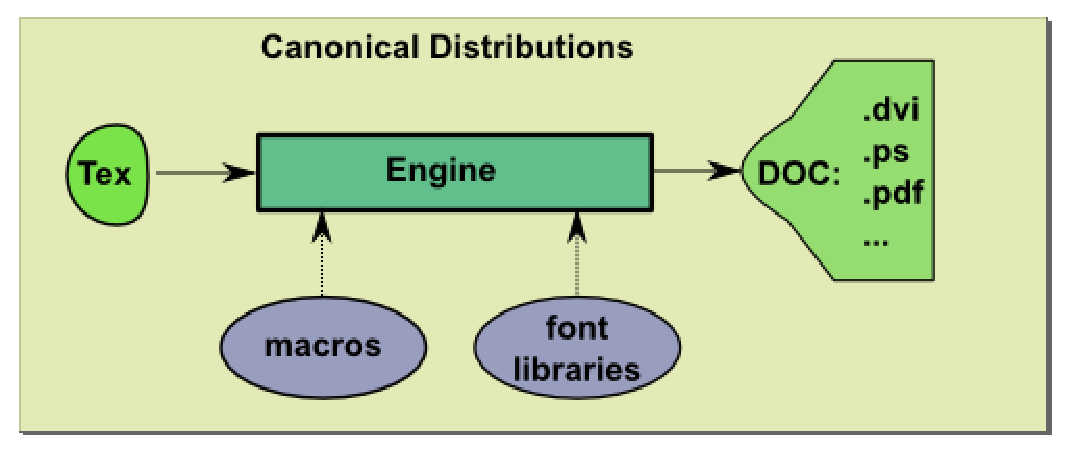
\includegraphics[scale=0.7]{figure/tex_engine}\caption[如果图题太长,在这里写个短标题只在图索引中出现]{\label{fig:tex_work_framework}\protect\TeX{}工作体系框架}
\end{figure}


用\LaTeX{}可以输入复杂的排版公式,如\eqref{eq:cx1}式。
\begin{equation}
\frac{\partial\,P(S_{j},\,t)}{\partial t}=\sum_{i}P(S_{i},\,t)W(S_{i}\rightarrow S_{j})-\sum_{i}P(S_{j},\,t)W(S_{j}\rightarrow S_{i})\label{eq:cx1}
\end{equation}


也可以输入表格如表 \ref{tab:example}。

\begin{table}
\caption{\label{tab:example}实例表}


\centering{}%
\begin{tabular}{c|c|c|c|c}
\hline 
case & Method1 & Method2 & Method3 & 产出\tabularnewline
\hline 
1 & 32 & 34 & 23 & 34\tabularnewline
\hline 
2 & 12 & 324 & 23 & 234\tabularnewline
\hline 
3 & 23 & 34 & 34 & 23\tabularnewline
\hline 
4 & 12 & 23 & 34 & 23\tabularnewline
\hline 
\end{tabular}
\end{table}



\subsection{关于\protect\LaTeX{}宏包的设计}

设计宏的源文件一般含.ins和.dtx两个文件,再调用\LaTeX{}工具命令生成.cls和.sty文件,当然我们可以直接设计.cls和.sty,无非.ins和.dtx多了一些安装说明和文档说明。

刚开始学\TeX{}和LATEX推荐阅读参考文献\cite{lshort,lamport1994latexa}。


\section{Lyx工具简介}

\LyX{}是一种半所见所得文档编辑工具,能够支持\TeX{}文档编辑。在\LyX{}主窗口输入用户文字内容,通过菜单命令将文档转换为\TeX{}格式,再在后台调用\LaTeX{}或其他引擎如Xe\LaTeX{}来编译成为最终文档。

\LyX{}的体系包含三大组成部分:
\begin{enumerate}
\item \TeX{}/\LaTeX{} 宏:\LyX{}会收集系统上已经存在的\TeX{}/\LaTeX{}宏,这些宏在\LyX{}的layout文件中调用。
\item 文档class\ and\ Layout:Layout主要规定\LyX{}用户输入界面文档显示的格式,这些格式没有必要和\LaTeX{}的生成格式但推荐一致。Linux系统下,在\textasciitilde{}/.lyx/layouts目录下可以定义自己的layout文件,可以通过菜单栏Document->settings->document\ class来选择。当前最新版可以在Document->settings->document\ class中使用“local\ layout”选择使用本地目录下的lyx\ layout文件,如“scutthesis.layout”。\LyX{}菜单上的help->customization\ layout的作用有两个:调用用户指定的tex\ class和设置\LyX{}文本界面段落格式。 
\item Template:其实就是一个正常的\LyX{}文件,作为一个模板,保存了一些相应的基本设置,这样你下次在需要此类格式的文档时,只要在该模板的基础上次新建即可。
\end{enumerate}
另外,如果你的要求不太高,完全可以把\LyX{}当成一个\LaTeX{}的草稿本,因为\LyX{}可以方便导出\LaTeX{}格式文档。


\chapter{结论}

本文研究了一种新颖的\LyX{}+Xe\LaTeX{}+\LaTeX{}组合的科技文献排版方式,设计了第一个专业型华南理工大学\LaTeX{}/\LyX{}博士学位论文模板库,在全国高校学位论文模板中,首创支持Lyx论文编辑,实现了模板使用与操作系统平台无关,一键生成pdf文件的快捷方式。

总体来说,\LyX{}、Xe\LaTeX{}和\LaTeX{}组合实现了一种优势互补,使得科技文献的编辑排版工作量大为下降。

\bibliographystyle{scutthesis}
\bibliography{scutthesis}



\appendix{附录}


\section{Ubuntu Linux系统下中文字体的安装}

\label{sec:ubuntuzhfont}

整个过程分为两部分:得到中文字体文件和安装设置。

File `algorithm2e.sty' not found. 

sudo apt-get install texlive-science

常用中文字体有三套:

1. winfonts(微软的六种中易字体,包括宋体、黑体、楷书、仿宋、隶书、幼圆),

2. adobefonts(Adobe 的四套字体,包括 Adobe Song Std、Adobe Heiti Std、Adobe
Fangsong Std、Adobe Kaiti Std)

3. Ubuntu开源的文泉字体

CTex宏库默认支持winfonts和adboefonts。因此要在linux系统下使用Ctex宏库最好是安装这些字库之一。

将要按照的字体放置到默认搜索路径\textasciitilde{}/.fonts中,运行fc-cache -fv 命令更新字体缓存,然后执行
fc-list :lang=zh查看是否有新安安装字体。

网络上有介绍http://blog.chinaunix.net/u3/109488/showart\_2222797.html

从windows系统中拷贝如下字体到 \textasciitilde{}/.fonts/winfonts 目录中。

\begin{lstlisting}[language=bash]
:~/.fonts/winfonts$ls
arialbd.ttf ARIALNB.TTF ariblk.ttf cour.ttf SIMLI.TTF timesbi.ttf
arialbi.ttf ARIALNI.TTF courbd.ttf simfang.ttf simsun.ttc timesi.ttf 
ariali.ttf ARIALN.TTF courbi.ttf simhei.ttf SIMYOU.TTF times.ttf
ARIALNBI.TTF arial.ttf couri.ttf simkai.ttf timesbd.ttf 
\end{lstlisting}


这样以后你的系统就安装好ctex需要的winfonts。(除此之外,上面的字体中还包含了Times New Roman、Arial、Courier
New英文字体) 

\emph{注意:}scutthesis.cls使用的是windows中文字体,在一般Linux没有带这些字体,需要自己安装。现有的字体库下载地址为:http://www.

在windows系统下,不需要下载安装这些字体,如果你使用的是其他windows版本的中文字体,编译scutthesis.ly或者scutthesis.tex时提示:



%\chapterx{攻读博士学位期间取得的研究成果}
%
%已发表(包括已接受待发表)的论文,以及已投稿、或已成文打算投稿、或拟成文投稿的论文情况(只填写与学位论文内容相关的部分):
%
%\begin{longtable}{|>{\centering}m{0.5cm}|>{\centering}m{2.3cm}|>{\centering}m{3.5cm}|>{\centering}m{2.6cm}|>{\centering}m{2cm}|>{\centering}m{1.3cm}|>{\centering}m{0.9cm}|}
%\hline 
%序号 & 作者(全体作者,按顺序排列) & 题 目 & 发表或投稿刊物名称、级别 & 发表的卷期、年月、页码 & 相当于学位论文的哪一部分(章、节) & 被索引收录情况\tabularnewline
%\hline 
%1 & 作者名 & 论文题目1 & 刊物名 & 发表时间 & 第2章 & SCI\tabularnewline
%\hline 
%2 & 作者名 & 论文题目2 & 刊物名 & 发表时间 & 第3章 & SCI\tabularnewline
%\hline 
% &  &  &  &  &  & \tabularnewline
%\hline 
% &  &  &  &  &  & \tabularnewline
%\hline 
% &  &  &  &  &  & \tabularnewline
%\hline 
% &  &  &  &  &  & \tabularnewline
%\hline 
%\end{longtable}
%
%
\chapterx{致谢}

感谢导师对我的悉心指导,同时感谢华工校内外多位同学对该模板的测试和提供的改进。

\begin{minipage}[t]{0.8\columnwidth}%
\begin{flushright}
姓名 
\par\end{flushright}

\begin{flushright}
2010年6月8日
\par\end{flushright}%
\end{minipage}
\end{document}
